\documentclass{article}
\usepackage{amsmath}
\usepackage{color,pxfonts,fix-cm}
\usepackage{latexsym}
\usepackage[mathletters]{ucs}
\DeclareUnicodeCharacter{32}{$\ $}
\usepackage[T1]{fontenc}
\usepackage[utf8x]{inputenc}
\usepackage{pict2e}
\usepackage{wasysym}
\usepackage[english]{babel}
\usepackage{tikz}
\pagestyle{empty}
\usepackage[margin=0in,paperwidth=612pt,paperheight=792pt]{geometry}
\begin{document}
\definecolor{color_29791}{rgb}{0,0,0}
\begin{tikzpicture}[overlay]\path(0pt,0pt);\end{tikzpicture}
\begin{picture}(-5,0)(2,0)[!]
\put(70.05,-76.258){\fontsize{14}{1}\usefont{T1}{cmr}{m}{n}\selectfont\color{color_29791}El }
\put(89.496,-76.258){\fontsize{14}{1}\usefont{T1}{cmr}{m}{n}\selectfont\color{color_29791}pr}
\put(105.036,-76.258){\fontsize{14}{1}\usefont{T1}{cmr}{m}{n}\selectfont\color{color_29791}oceso }
\put(155.618,-76.258){\fontsize{14}{1}\usefont{T1}{cmr}{m}{n}\selectfont\color{color_29791}realizado para }
\put(269.2,-76.258){\fontsize{14}{1}\usefont{T1}{cmr}{m}{n}\selectfont\color{color_29791}la conversión de }
\put(399.89,-76.258){\fontsize{14}{1}\usefont{T1}{cmr}{m}{n}\selectfont\color{color_29791}la formula }
\put(70.05,-97.56195){\fontsize{14}{1}\usefont{T1}{cmr}{m}{n}\selectfont\color{color_29791}Simpson a }
\put(154.064,-97.56195){\fontsize{14}{1}\usefont{T1}{cmr}{m}{n}\selectfont\color{color_29791}un código}
\put(228.768,-97.56195){\fontsize{14}{1}\usefont{T1}{cmr}{m}{n}\selectfont\color{color_29791} funcional }
\put(308.904,-97.56195){\fontsize{14}{1}\usefont{T1}{cmr}{m}{n}\selectfont\color{color_29791}con su }
\put(364.148,-97.56195){\fontsize{14}{1}\usefont{T1}{cmr}{m}{n}\selectfont\color{color_29791}r}
\put(370.35,-97.56195){\fontsize{14}{1}\usefont{T1}{cmr}{m}{n}\selectfont\color{color_29791}espectiva prueba.}
\put(70.05,-122.661){\fontsize{12}{1}\usefont{T1}{ptm}{m}{n}\selectfont\color{color_29791}Para come}
\put(120.354,-122.661){\fontsize{12}{1}\usefont{T1}{ptm}{m}{n}\selectfont\color{color_29791}nzar se anali}
\put(180.318,-122.661){\fontsize{12}{1}\usefont{T1}{ptm}{m}{n}\selectfont\color{color_29791}zó que informac}
\put(258.282,-122.661){\fontsize{12}{1}\usefont{T1}{ptm}{m}{n}\selectfont\color{color_29791}ión que se iba a usar pa}
\put(370.242,-122.661){\fontsize{12}{1}\usefont{T1}{ptm}{m}{n}\selectfont\color{color_29791}ra la impl}
\put(416.226,-122.661){\fontsize{12}{1}\usefont{T1}{ptm}{m}{n}\selectfont\color{color_29791}ementac}
\put(456.198,-122.661){\fontsize{12}{1}\usefont{T1}{ptm}{m}{n}\selectfont\color{color_29791}ión en el }
\put(70.05,-137.552){\fontsize{12}{1}\usefont{T1}{ptm}{m}{n}\selectfont\color{color_29791}código el}
\put(114.366,-137.552){\fontsize{12}{1}\usefont{T1}{ptm}{m}{n}\selectfont\color{color_29791} cual fue proveí}
\put(189.33,-137.552){\fontsize{12}{1}\usefont{T1}{ptm}{m}{n}\selectfont\color{color_29791}do en un documento}
\put(286.974,-137.552){\fontsize{12}{1}\usefont{T1}{ptm}{m}{n}\selectfont\color{color_29791} pdf por el maestro Cent}
\put(403.278,-137.552){\fontsize{12}{1}\usefont{T1}{ptm}{m}{n}\selectfont\color{color_29791}eno en el cua}
\put(466.242,-137.552){\fontsize{12}{1}\usefont{T1}{ptm}{m}{n}\selectfont\color{color_29791}l }
\put(70.05,-152.443){\fontsize{12}{1}\usefont{T1}{ptm}{m}{n}\selectfont\color{color_29791}contení}
\put(105.366,-152.443){\fontsize{12}{1}\usefont{T1}{ptm}{m}{n}\selectfont\color{color_29791}a tanto una e}
\put(166.338,-152.443){\fontsize{12}{1}\usefont{T1}{ptm}{m}{n}\selectfont\color{color_29791}xplicaci}
\put(204.318,-152.443){\fontsize{12}{1}\usefont{T1}{ptm}{m}{n}\selectfont\color{color_29791}ón de el cómo func}
\put(296.286,-152.443){\fontsize{12}{1}\usefont{T1}{ptm}{m}{n}\selectfont\color{color_29791}iona la formul}
\put(364.266,-152.443){\fontsize{12}{1}\usefont{T1}{ptm}{m}{n}\selectfont\color{color_29791}a desglosando paso a paso la }
\put(70.05,-167.334){\fontsize{12}{1}\usefont{T1}{ptm}{m}{n}\selectfont\color{color_29791}misma}
\put(102.042,-167.334){\fontsize{12}{1}\usefont{T1}{ptm}{m}{n}\selectfont\color{color_29791} los cuales eran:}
\put(70,-320.334){\fontsize{12}{1}\usefont{T1}{ptm}{m}{n}\selectfont\color{color_29791} 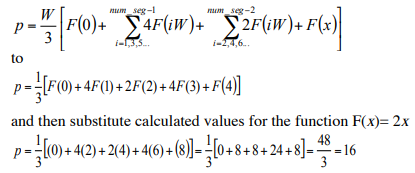
\includegraphics[width=15cm, height=5cm]{Formula.png}
}
\put(70.05,-329.817){\fontsize{12}{1}\usefont{T1}{ptm}{m}{n}\selectfont\color{color_29791}Una vez conoc}
\put(141.342,-329.817){\fontsize{12}{1}\usefont{T1}{ptm}{m}{n}\selectfont\color{color_29791}ida la formul}
\put(203.322,-329.817){\fontsize{12}{1}\usefont{T1}{ptm}{m}{n}\selectfont\color{color_29791}a a util}
\put(235.974,-329.817){\fontsize{12}{1}\usefont{T1}{ptm}{m}{n}\selectfont\color{color_29791}izar se comenz}
\put(307.266,-329.817){\fontsize{12}{1}\usefont{T1}{ptm}{m}{n}\selectfont\color{color_29791}aría el de}
\put(351.234,-329.817){\fontsize{12}{1}\usefont{T1}{ptm}{m}{n}\selectfont\color{color_29791}s}
\put(355.914,-329.817){\fontsize{12}{1}\usefont{T1}{ptm}{m}{n}\selectfont\color{color_29791}gl}
\put(365.238,-329.817){\fontsize{12}{1}\usefont{T1}{ptm}{m}{n}\selectfont\color{color_29791}os}
\put(375.918,-329.817){\fontsize{12}{1}\usefont{T1}{ptm}{m}{n}\selectfont\color{color_29791}e}
\put(381.234,-329.817){\fontsize{12}{1}\usefont{T1}{ptm}{m}{n}\selectfont\color{color_29791} de la misma}
\put(442.218,-329.817){\fontsize{12}{1}\usefont{T1}{ptm}{m}{n}\selectfont\color{color_29791} para nuestra }
\put(70.05,-344.708){\fontsize{12}{1}\usefont{T1}{ptm}{m}{n}\selectfont\color{color_29791}clase se l}
\put(113.358,-344.708){\fontsize{12}{1}\usefont{T1}{ptm}{m}{n}\selectfont\color{color_29791}a herramie}
\put(164.322,-344.708){\fontsize{12}{1}\usefont{T1}{ptm}{m}{n}\selectfont\color{color_29791}nta Excel}
\put(209.298,-344.708){\fontsize{12}{1}\usefont{T1}{ptm}{m}{n}\selectfont\color{color_29791} con el fin de pode}
\put(298.266,-344.708){\fontsize{12}{1}\usefont{T1}{ptm}{m}{n}\selectfont\color{color_29791}r clasifica}
\put(345.234,-344.708){\fontsize{12}{1}\usefont{T1}{ptm}{m}{n}\selectfont\color{color_29791}r y de esta forma poder}
\put(456.186,-344.708){\fontsize{12}{1}\usefont{T1}{ptm}{m}{n}\selectfont\color{color_29791} }
\put(70.05,-359.599){\fontsize{12}{1}\usefont{T1}{ptm}{m}{n}\selectfont\color{color_29791}aprovecha}
\put(119.346,-359.599){\fontsize{12}{1}\usefont{T1}{ptm}{m}{n}\selectfont\color{color_29791}r las herramie}
\put(185.31,-359.599){\fontsize{12}{1}\usefont{T1}{ptm}{m}{n}\selectfont\color{color_29791}ntas que la plat}
\put(257.622,-359.599){\fontsize{12}{1}\usefont{T1}{ptm}{m}{n}\selectfont\color{color_29791}aforma ofrece}
\put(70.05,-550){\fontsize{12}{1}\usefont{T1}{ptm}{m}{n}\selectfont\color{color_29791} 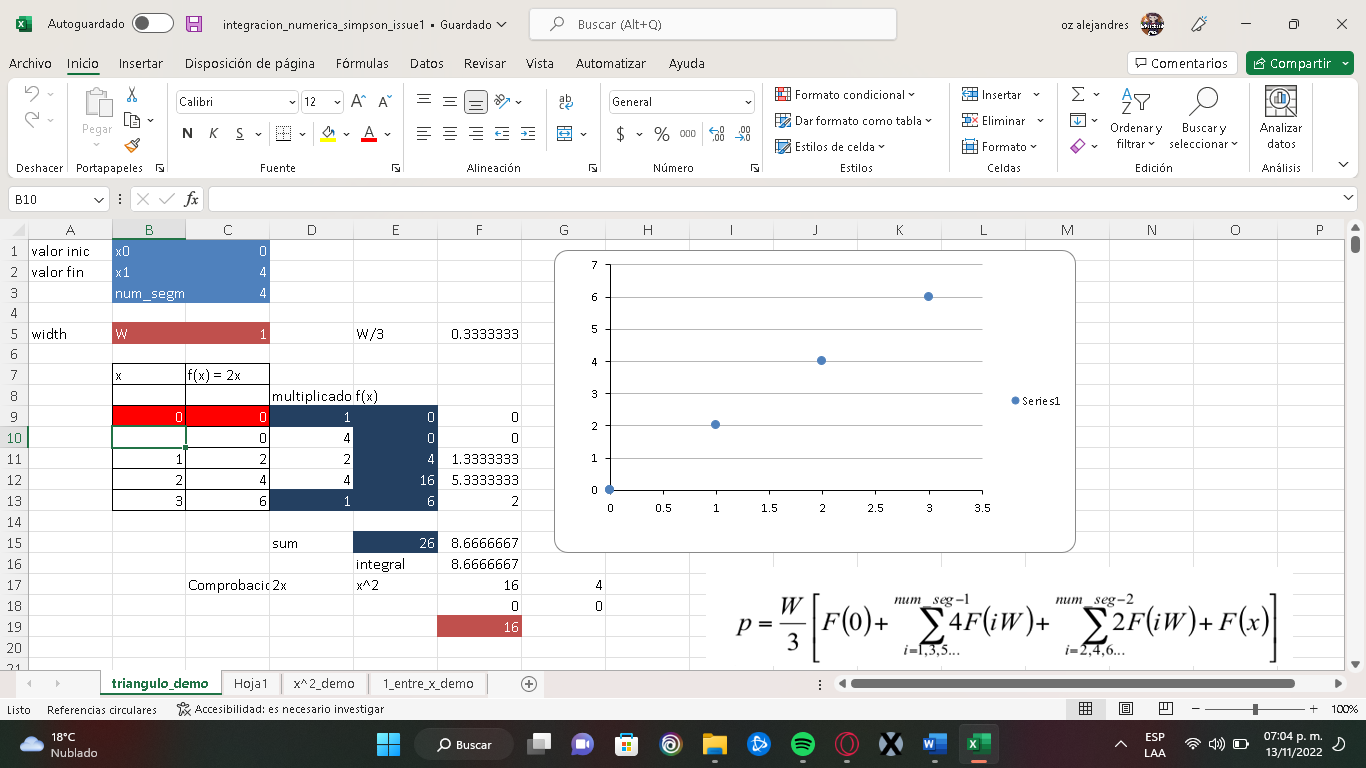
\includegraphics[width=14cm, height=6cm]{Cuadros.png}}
\put(70.05,-598.082){\fontsize{12}{1}\usefont{T1}{ptm}{m}{n}\selectfont\color{color_29791} En la}
\put(98.034,-598.082){\fontsize{12}{1}\usefont{T1}{ptm}{m}{n}\selectfont\color{color_29791} cual se desgloso punto por punto l}
\put(265.014,-598.082){\fontsize{12}{1}\usefont{T1}{ptm}{m}{n}\selectfont\color{color_29791}as operaciones que la}
\put(367.302,-598.082){\fontsize{12}{1}\usefont{T1}{ptm}{m}{n}\selectfont\color{color_29791} formula requerí}
\put(445.266,-598.082){\fontsize{12}{1}\usefont{T1}{ptm}{m}{n}\selectfont\color{color_29791}an para }
\put(70.05,-612.973){\fontsize{12}{1}\usefont{T1}{ptm}{m}{n}\selectfont\color{color_29791}comenz}
\put(107.358,-612.973){\fontsize{12}{1}\usefont{T1}{ptm}{m}{n}\selectfont\color{color_29791}ar el proceso se com}
\put(205.314,-612.973){\fontsize{12}{1}\usefont{T1}{ptm}{m}{n}\selectfont\color{color_29791}enzó por trabaj}
\put(277.278,-612.973){\fontsize{12}{1}\usefont{T1}{ptm}{m}{n}\selectfont\color{color_29791}ar con el valor}
\put(346.242,-612.973){\fontsize{12}{1}\usefont{T1}{ptm}{m}{n}\selectfont\color{color_29791} X}
\put(357.918,-612.973){\fontsize{12}{1}\usefont{T1}{ptm}{m}{n}\selectfont\color{color_29791}0, X1 y num\_segm}
\put(70.05,-635.864){\fontsize{12}{1}\usefont{T1}{ptm}{m}{n}\selectfont\color{color_29791}Posteriorment}
\put(137.37,-635.864){\fontsize{12}{1}\usefont{T1}{ptm}{m}{n}\selectfont\color{color_29791}e se comenza}
\put(201.33,-635.864){\fontsize{12}{1}\usefont{T1}{ptm}{m}{n}\selectfont\color{color_29791}ría el ca}
\put(239.298,-635.864){\fontsize{12}{1}\usefont{T1}{ptm}{m}{n}\selectfont\color{color_29791}lculo de los val}
\put(312.282,-635.864){\fontsize{12}{1}\usefont{T1}{ptm}{m}{n}\selectfont\color{color_29791}ores X}
\put(343.95,-635.864){\fontsize{12}{1}\usefont{T1}{ptm}{m}{n}\selectfont\color{color_29791} y f(x) = 2x y de}
\put(422.022,-635.864){\fontsize{12}{1}\usefont{T1}{ptm}{m}{n}\selectfont\color{color_29791}s}
\put(426.702,-635.864){\fontsize{12}{1}\usefont{T1}{ptm}{m}{n}\selectfont\color{color_29791}pué}
\put(444.018,-635.864){\fontsize{12}{1}\usefont{T1}{ptm}{m}{n}\selectfont\color{color_29791}s}
\put(448.698,-635.864){\fontsize{12}{1}\usefont{T1}{ptm}{m}{n}\selectfont\color{color_29791} }
\put(70.05,-650.7549){\fontsize{12}{1}\usefont{T1}{ptm}{m}{n}\selectfont\color{color_29791}mult}
\put(92.04601,-650.7549){\fontsize{12}{1}\usefont{T1}{ptm}{m}{n}\selectfont\color{color_29791}iplicarlos y sumar l}
\put(184.362,-650.7549){\fontsize{12}{1}\usefont{T1}{ptm}{m}{n}\selectfont\color{color_29791}os}
\put(195.042,-650.7549){\fontsize{12}{1}\usefont{T1}{ptm}{m}{n}\selectfont\color{color_29791} re}
\put(207.354,-650.7549){\fontsize{12}{1}\usefont{T1}{ptm}{m}{n}\selectfont\color{color_29791}s}
\put(212.034,-650.7549){\fontsize{12}{1}\usefont{T1}{ptm}{m}{n}\selectfont\color{color_29791}ul}
\put(221.358,-650.7549){\fontsize{12}{1}\usefont{T1}{ptm}{m}{n}\selectfont\color{color_29791}tados obtenidos todos los cál}
\put(359.346,-650.7549){\fontsize{12}{1}\usefont{T1}{ptm}{m}{n}\selectfont\color{color_29791}culos realiz}
\put(414.318,-650.7549){\fontsize{12}{1}\usefont{T1}{ptm}{m}{n}\selectfont\color{color_29791}ados fueron hechos }
\put(70.05,-665.6459){\fontsize{12}{1}\usefont{T1}{ptm}{m}{n}\selectfont\color{color_29791}con el fi}
\put(109.362,-665.6459){\fontsize{12}{1}\usefont{T1}{ptm}{m}{n}\selectfont\color{color_29791}n de poder obtener}
\put(198.99,-665.6459){\fontsize{12}{1}\usefont{T1}{ptm}{m}{n}\selectfont\color{color_29791} una gráfica que pue}
\put(296.274,-665.6459){\fontsize{12}{1}\usefont{T1}{ptm}{m}{n}\selectfont\color{color_29791}da determi}
\put(347.25,-665.6459){\fontsize{12}{1}\usefont{T1}{ptm}{m}{n}\selectfont\color{color_29791}nar si dichos resultados son }
\put(70.05,-680.5369){\fontsize{12}{1}\usefont{T1}{ptm}{m}{n}\selectfont\color{color_29791}confiabl}
\put(109.362,-680.5369){\fontsize{12}{1}\usefont{T1}{ptm}{m}{n}\selectfont\color{color_29791}es todos los resultados deberán ba}
\put(272.322,-680.5369){\fontsize{12}{1}\usefont{T1}{ptm}{m}{n}\selectfont\color{color_29791}s}
\put(277.002,-680.5369){\fontsize{12}{1}\usefont{T1}{ptm}{m}{n}\selectfont\color{color_29791}a}
\put(282.318,-680.5369){\fontsize{12}{1}\usefont{T1}{ptm}{m}{n}\selectfont\color{color_29791}rs}
\put(290.994,-680.5369){\fontsize{12}{1}\usefont{T1}{ptm}{m}{n}\selectfont\color{color_29791}e}
\put(296.31,-680.5369){\fontsize{12}{1}\usefont{T1}{ptm}{m}{n}\selectfont\color{color_29791} en la tabl}
\put(343.29,-680.5369){\fontsize{12}{1}\usefont{T1}{ptm}{m}{n}\selectfont\color{color_29791}a que el mi}
\put(396.27,-680.5369){\fontsize{12}{1}\usefont{T1}{ptm}{m}{n}\selectfont\color{color_29791}s}
\put(400.95,-680.5369){\fontsize{12}{1}\usefont{T1}{ptm}{m}{n}\selectfont\color{color_29791}m}
\put(410.274,-680.5369){\fontsize{12}{1}\usefont{T1}{ptm}{m}{n}\selectfont\color{color_29791}o documento }
\end{picture}
\newpage
\begin{tikzpicture}[overlay]\path(0pt,0pt);\end{tikzpicture}
\begin{picture}(-5,0)(2.5,0)
\put(70.05,-72.05298){\fontsize{12}{1}\usefont{T1}{ptm}{m}{n}\selectfont\color{color_29791}proporcionado m}
\put(152.358,-72.05298){\fontsize{12}{1}\usefont{T1}{ptm}{m}{n}\selectfont\color{color_29791}uestra para poder t}
\put(241.314,-72.05298){\fontsize{12}{1}\usefont{T1}{ptm}{m}{n}\selectfont\color{color_29791}rabajar tant}
\put(295.614,-72.05298){\fontsize{12}{1}\usefont{T1}{ptm}{m}{n}\selectfont\color{color_29791}o el código com}
\put(372.594,-72.05298){\fontsize{12}{1}\usefont{T1}{ptm}{m}{n}\selectfont\color{color_29791}o las pruebas que buscaran }
\put(70.05,-86.94397){\fontsize{12}{1}\usefont{T1}{ptm}{m}{n}\selectfont\color{color_29791}obtener}
\put(106.026,-86.94397){\fontsize{12}{1}\usefont{T1}{ptm}{m}{n}\selectfont\color{color_29791} }
\put(109.038,-86.94397){\fontsize{12}{1}\usefont{T1}{ptm}{m}{n}\selectfont\color{color_29791}u}
\put(115.026,-86.94397){\fontsize{12}{1}\usefont{T1}{ptm}{m}{n}\selectfont\color{color_29791}n}
\put(121.038,-86.94397){\fontsize{12}{1}\usefont{T1}{ptm}{m}{n}\selectfont\color{color_29791}o}
\put(127.026,-86.94397){\fontsize{12}{1}\usefont{T1}{ptm}{m}{n}\selectfont\color{color_29791}s}
\put(131.706,-86.94397){\fontsize{12}{1}\usefont{T1}{ptm}{m}{n}\selectfont\color{color_29791} result}
\put(161.358,-86.94397){\fontsize{12}{1}\usefont{T1}{ptm}{m}{n}\selectfont\color{color_29791}ados concretos.}
\put(70.05,-350){\fontsize{12}{1}\usefont{T1}{ptm}{m}{n}\selectfont\color{color_29791} 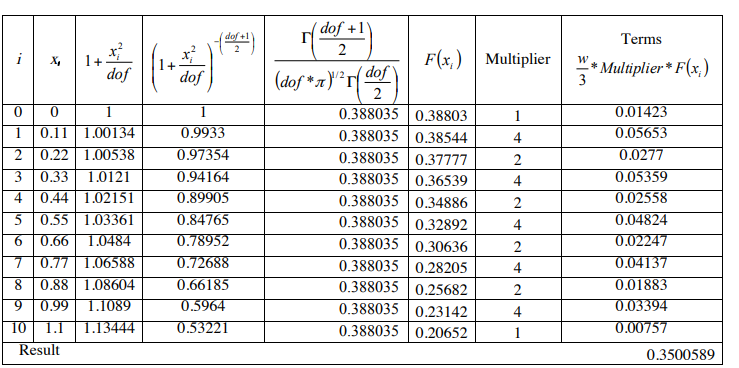
\includegraphics[width=14cm, height=9cm]{Datos.png}}
\put(70.05,-362.527){\fontsize{12}{1}\usefont{T1}{ptm}{m}{n}\selectfont\color{color_29791}El obj}
\put(99.04201,-362.527){\fontsize{12}{1}\usefont{T1}{ptm}{m}{n}\selectfont\color{color_29791}etivo de la}
\put(149.022,-362.527){\fontsize{12}{1}\usefont{T1}{ptm}{m}{n}\selectfont\color{color_29791} f}
\put(156.03,-362.527){\fontsize{12}{1}\usefont{T1}{ptm}{m}{n}\selectfont\color{color_29791}orm}
\put(175.35,-362.527){\fontsize{12}{1}\usefont{T1}{ptm}{m}{n}\selectfont\color{color_29791}ula es obtener}
\put(241.986,-362.527){\fontsize{12}{1}\usefont{T1}{ptm}{m}{n}\selectfont\color{color_29791} una curva basado en l}
\put(348.942,-362.527){\fontsize{12}{1}\usefont{T1}{ptm}{m}{n}\selectfont\color{color_29791}a formula Simpson con l}
\put(466.926,-362.527){\fontsize{12}{1}\usefont{T1}{ptm}{m}{n}\selectfont\color{color_29791}a cual }
\put(70.05,-377.418){\fontsize{12}{1}\usefont{T1}{ptm}{m}{n}\selectfont\color{color_29791}los datos obteni}
\put(145.374,-377.418){\fontsize{12}{1}\usefont{T1}{ptm}{m}{n}\selectfont\color{color_29791}dos}
\put(162.054,-377.418){\fontsize{12}{1}\usefont{T1}{ptm}{m}{n}\selectfont\color{color_29791} que}
\put(182.37,-377.418){\fontsize{12}{1}\usefont{T1}{ptm}{m}{n}\selectfont\color{color_29791} queden dentro de}
\put(268.002,-377.418){\fontsize{12}{1}\usefont{T1}{ptm}{m}{n}\selectfont\color{color_29791} la curva basado en}
\put(359.958,-377.418){\fontsize{12}{1}\usefont{T1}{ptm}{m}{n}\selectfont\color{color_29791} una distribución de}
\put(454.938,-377.418){\fontsize{12}{1}\usefont{T1}{ptm}{m}{n}\selectfont\color{color_29791} bloques se }
\put(70.05,-392.309){\fontsize{12}{1}\usefont{T1}{ptm}{m}{n}\selectfont\color{color_29791}puedan det}
\put(122.358,-392.309){\fontsize{12}{1}\usefont{T1}{ptm}{m}{n}\selectfont\color{color_29791}erminar cuá}
\put(179.322,-392.309){\fontsize{12}{1}\usefont{T1}{ptm}{m}{n}\selectfont\color{color_29791}nto es el marge}
\put(252.294,-392.309){\fontsize{12}{1}\usefont{T1}{ptm}{m}{n}\selectfont\color{color_29791}n de error de los datos proporci}
\put(402.246,-392.309){\fontsize{12}{1}\usefont{T1}{ptm}{m}{n}\selectfont\color{color_29791}onados }
\end{picture}
\end{document}
\end{document}